\documentclass[a4paper,12pt]{article}
\usepackage[utf8]{inputenc}
\usepackage[english]{babel}
\usepackage{graphicx}
\usepackage{multicol}  
\usepackage{float}
\usepackage{csquotes}
\usepackage{hyperref}
\hypersetup{
    colorlinks=true,
    linkcolor=black,
    filecolor=black,      
    urlcolor=black,
    citecolor=black,
}

\usepackage{biblatex}
\addbibresource{ipk.bib}

\begin{document}
 \pagenumbering{alph}
\begin{titlepage}
    \begin{center}

        
\includegraphics[width=\linewidth]{logo.jpg}
        \vspace*{0.5cm}
            
        \Huge
        \textbf{Project Documentation}
            
        \vspace{0.5cm}
        \LARGE
        Computer Communications and Networks
        
            
        \vspace{1.5cm}
            
        \textbf{Lukáš Foltyn}
            
        \vfill
        Zeta - Packet sniffer\\
        2020/2021
            
        \vspace{0.8cm}
 
    \end{center}
\end{titlepage}
\pagenumbering{arabic}
\tableofcontents{}
\newpage
\frenchspacing

\section{Introduction}
    \subsection{Project description}
    The goal of this project was to implement a light version of packet sniffer. Task has been given in Computer Communications and Networks course at VUT Faculty of information technology. 
    
    \subsection{Project structure}
    Project consists of four source code files. The \texttt{ipk-sniffer.cpp}'s functionality is mostly to parse command line arguments and catch the raw packets, that are parsed in \texttt{PacketInfo} class that is declared in \texttt{packet\_info.h} and defined in \texttt{packet\_info.cpp}. For its correct functionality are used structures that can be found in \texttt{defined\_headers.h}.
    
\section{Implementation}
    Packet sniffer is implemented in C\texttt{++} language. For parsing command line arguments is used a \texttt{getopt} function \cite{getopt}. For getting correct offsets in array of bytes (representing a given packet) are used structures from a network header files: \texttt{netinet/}\{\texttt{ip, in, tcp, udp, ip\_icmp, ip6, if\_ether}\}\texttt{.h}. Catching user's CTRL\texttt{+}C termination signal is handled by functions from \texttt{signal.h}, so that the program ends correctly even when unexpected and forced termination is required. Lastly but most importantly, for capturing the packets was installed a libcap library \cite{tcpdump}, which provides a wide variety of functions to do so. Here is the list of used libcap functions:
    \begin{multicols}{2}
    \begin{itemize}
        \item \href{https://man7.org/linux/man-pages/man3/pcap_findalldevs.3pcap.html}{\texttt{pcap\_findalldevs()}}
        \item \href{https://linux.die.net/man/3/pcap_freealldevs}{\texttt{pcap\_freealldevs()}}
        \item \href{https://linux.die.net/man/3/pcap_open_live}{\texttt{pcap\_open\_live()}}
        \item \href{https://linux.die.net/man/3/pcap_lookupnet}{\texttt{pcap\_lookupnet()}}
        \item \href{https://linux.die.net/man/3/pcap_compile}{\texttt{pcap\_compile()}}
    \end{itemize}
    \columnbreak
    \begin{itemize}
        \item \href{https://man7.org/linux/man-pages/man3/pcap_setfilter.3pcap.html}{\texttt{pcap\_setfilter()}}
        \item \href{https://linux.die.net/man/3/pcap_loop}{\texttt{pcap\_loop()}}
        \item \href{https://man7.org/linux/man-pages/man3/pcap_geterr.3pcap.html}{\texttt{pcap\_geterr()}}
        \item \href{https://man7.org/linux/man-pages/man3/pcap_freecode.3pcap.html}{\texttt{pcap\_freecode()}}
        \item \href{https://linux.die.net/man/3/pcap_close}{\texttt{pcap\_close()}}
    \end{itemize}
    \end{multicols}
    \newpage
    \subsection{PacketInfo class and its functions}
        Class consisting of nine functions, that are able to find a particular information contained in the packet and one function that prints out the whole packet with all desired info. It only needs a pointer to packet data and a pointer to \texttt{pcap\_pkthrd} structure that holds the information about packet lenght as well as the time when the packet was received.
        \subsubsection{get\_network\_protocol()}
        Finds out what kind of network protocol follows after the data link layer. Works only if a given packet has ethernet header, which means 14 bytes offset from the beginning of the packet. 
        
        \subsubsection{get\_transport\_protocol()}
        Finds out what kind of transport protocol follows after the network layer. Both IPv4 and IPv6 are supported as network protocols. Even extension headers are allowed. This functionality is done by looping through headers until a transport protocol header is reached or exception is thrown if unexpected protocol occurs. 
        
        \subsubsection{get\_network\_header()}
        Searches for the position in the packet where a network protocol header starts and returns a pointer to it. Again, as in \texttt{get\_network\_protocol()} function, this works only with ethernet header.
        
        \subsubsection{get\_transport\_header()}
        Searches for the position in the packet where a transport protocol header starts. Works exactly the same way as a \texttt{get\_transport\_protocol()} function, but instead of protocol type, pointer to a transport protocol header is returned.
        
        \subsubsection{get\_source\_ip() and get\_destination\_ip()}
        Functions that find and return source/destination ip address
        contained in the packet if it's valid, otherwise an exception is thrown. Both class functions \texttt{get\_network\_}\{\texttt{protocol/header}\} are used here. Ip addresses are converted into a correct format with help of \texttt{inet\_ntoa()} function for IPv4, \texttt{inet\_ntop()} function for IPv6. From \textbf{ARP} packets the \textbf{sender/target} ip address is obtained by bitwise operations.
        
        \subsubsection{get\_source\_port() and get\_destination\_port()}
        Functions that find and return source/destination port contained in the packet if it's valid, otherwise an exception is thrown. Two more class functions are used here - \texttt{get\_transport\_header()} and \texttt{get\_transport\_protocol()}. In this case, valid protocols
        are TCP and UDP.
                
        \subsubsection{get\_timestamp()}
        Looks into the \texttt{pcap\_pkthrd} structure for the time when the packet was received and returns it converted in a RFC3339 format \cite{rfc}.
        
        \subsubsection{print\_packet()}
        This function is used for printing the whole packet in a similar format as Wireshark \cite{wireshark}. On the first line we can found time when the packet was received then source ip address/port followed by destination ip address/port and the length of the captured packet. Then the packet data are printed from the first to the last byte in hexadecimal format on the left side as well as in ASCII format on the right side. Non-printable characters are replaced with dot. 
        
        \begin{figure}[h]
            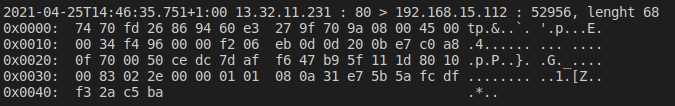
\includegraphics[width=\linewidth]{packet_example.png}
            \caption{Example of captured packet and its format}
        \end{figure}

\section{Testing}
This project was not tested by any other program or script. In this case, more of a static testing approach was chosen. Both \textbf{ipk-sniffer} and \textbf{Wireshark} were run and with the help of a small python script, different kinds of packets were generated and sent. Then the outputs were compared. You can see some examples on the next pages.
\newpage
\begin{figure}[H]

            \vfill
            
            \begin{center}

            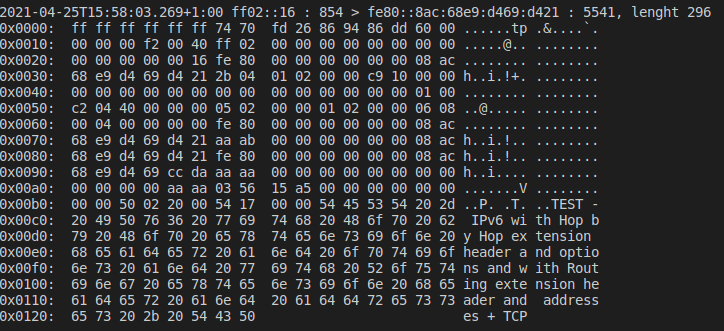
\includegraphics[width=\linewidth]{cmp1ipk.png}
            
            \vspace{0.5cm}
            
            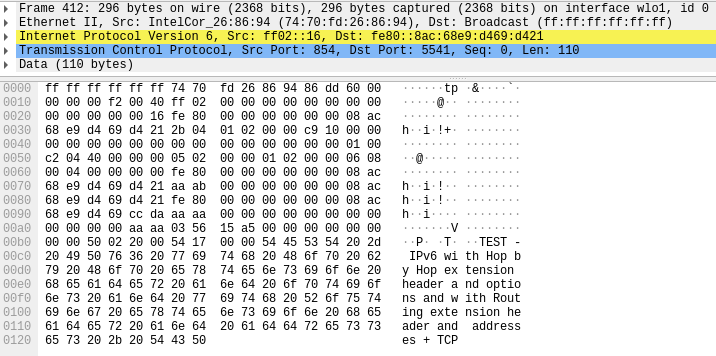
\includegraphics[width=\linewidth]{cmp1wireshark.png}
            \caption{IPv6/TCP packet with extension headers}
            \end{center}
            
            \vfill
            
\end{figure}

\begin{figure}[H]
            \vfill
            
            \begin{center}

            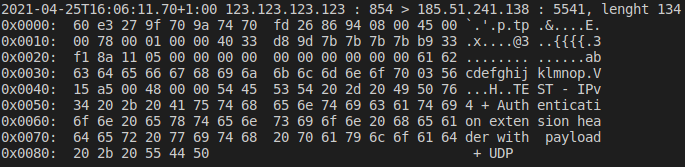
\includegraphics[width=\linewidth]{cmp2ipk.png}
            
            \vspace{0.5cm}
            
            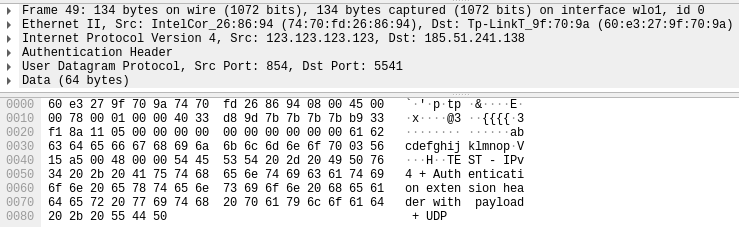
\includegraphics[width=\linewidth]{cmp2wireshark.png}
            \caption{IPv4/UDP packet with authentication header}
            \end{center}
            
            \vfill
\end{figure}

\begin{figure}[H]
            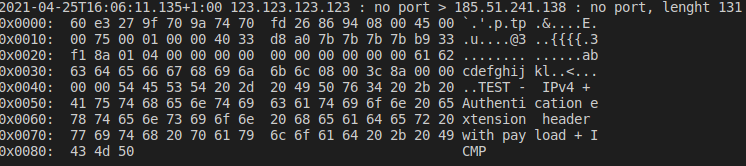
\includegraphics[width=\linewidth]{cmp3ipk.png}
            
            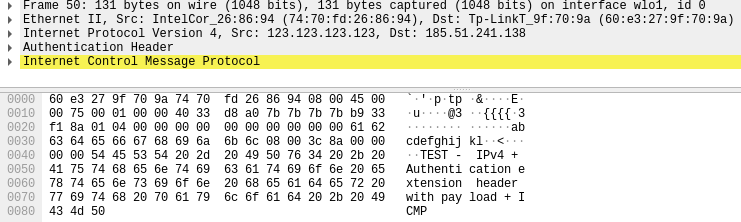
\includegraphics[width=\linewidth]{cmp3wireshark.png}
            \caption{IPv4/ICMP packet with authentication headers}
\end{figure}

\begin{figure}[H]
            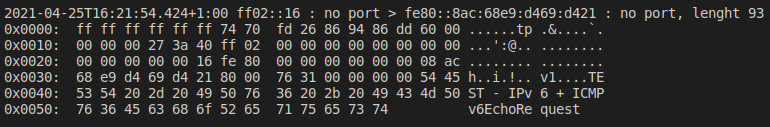
\includegraphics[width=\linewidth]{cmp4ipk.png}
            
            \vspace{0.5cm}
            
            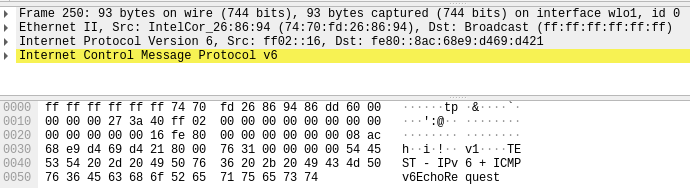
\includegraphics[width=\linewidth]{cmp4wireshark.png}
            
            \caption{IPv6/ICMPv6 packet}
\end{figure}


\nocite{ip6}
\nocite{filter}
\nocite{prg}
\nocite{sniff}
\nocite{arp}
\printbibliography

\end{document}
